\documentclass[rusmathsym, eqnumwithinsec, amspack, hyperref]{bomgost}

\DeclareTextSymbol{\CYRA}\UnicodeEncodingName{"0410}        % А
\DeclareTextSymbol{\cyra}\UnicodeEncodingName{"0430}        % а
\DeclareTextSymbol{\CYRB}\UnicodeEncodingName{"0411}        % Б
\DeclareTextSymbol{\cyrb}\UnicodeEncodingName{"0431}        % б
\DeclareTextSymbol{\CYRV}\UnicodeEncodingName{"0412}        % В 
\DeclareTextSymbol{\cyrv}\UnicodeEncodingName{"0432}        % в
\DeclareTextSymbol{\CYRG}\UnicodeEncodingName{"0413}        % Г
\DeclareTextSymbol{\cyrg}\UnicodeEncodingName{"0433}        % г
\DeclareTextSymbol{\CYRD}\UnicodeEncodingName{"0414}        % Д
\DeclareTextSymbol{\cyrd}\UnicodeEncodingName{"0434}        % д
\DeclareTextSymbol{\CYRE}\UnicodeEncodingName{"0415}        % Е 
\DeclareTextSymbol{\cyre}\UnicodeEncodingName{"0435}        % е
\DeclareTextSymbol{\CYRZH}\UnicodeEncodingName{"0416}       % Ж 
\DeclareTextSymbol{\cyrzh}\UnicodeEncodingName{"0436}       % ж
\DeclareTextSymbol{\CYRZ}\UnicodeEncodingName{"0417}        % З
\DeclareTextSymbol{\cyrz}\UnicodeEncodingName{"0437}        % з
\DeclareTextSymbol{\CYRI}\UnicodeEncodingName{"0418}        % И
\DeclareTextSymbol{\cyri}\UnicodeEncodingName{"0438}        % и
\DeclareTextSymbol{\CYRISHRT}\UnicodeEncodingName{"0419}    % Й
\DeclareTextSymbol{\cyrishrt}\UnicodeEncodingName{"0439}    % й
\DeclareTextSymbol{\CYRK}\UnicodeEncodingName{"041A}        % К
\DeclareTextSymbol{\cyrk}\UnicodeEncodingName{"043A}        % к
\DeclareTextSymbol{\CYRL}\UnicodeEncodingName{"041B}        % Л
\DeclareTextSymbol{\cyrl}\UnicodeEncodingName{"043B}        % л 
\DeclareTextSymbol{\CYRM}\UnicodeEncodingName{"041C}        % М
\DeclareTextSymbol{\cyrm}\UnicodeEncodingName{"043C}        % м
\DeclareTextSymbol{\CYRN}\UnicodeEncodingName{"041D}        % Н
\DeclareTextSymbol{\cyrn}\UnicodeEncodingName{"043D}        % н
\DeclareTextSymbol{\CYRO}\UnicodeEncodingName{"041E}        % О
\DeclareTextSymbol{\cyro}\UnicodeEncodingName{"043E}        % о
\DeclareTextSymbol{\CYRP}\UnicodeEncodingName{"041F}        % П
\DeclareTextSymbol{\cyrp}\UnicodeEncodingName{"043F}        % п
\DeclareTextSymbol{\CYRR}\UnicodeEncodingName{"0420}        % Р
\DeclareTextSymbol{\cyrr}\UnicodeEncodingName{"0440}        % р
\DeclareTextSymbol{\CYRS}\UnicodeEncodingName{"0421}        % С
\DeclareTextSymbol{\cyrs}\UnicodeEncodingName{"0441}        % с
\DeclareTextSymbol{\CYRT}\UnicodeEncodingName{"0422}        % Т
\DeclareTextSymbol{\cyrt}\UnicodeEncodingName{"0442}        % т
\DeclareTextSymbol{\CYRU}\UnicodeEncodingName{"0423}        % У
\DeclareTextSymbol{\cyru}\UnicodeEncodingName{"0443}        % у
\DeclareTextSymbol{\CYRF}\UnicodeEncodingName{"0424}        % Ф
\DeclareTextSymbol{\cyrf}\UnicodeEncodingName{"0444}        % ф
\DeclareTextSymbol{\CYRH}\UnicodeEncodingName{"0425}        % Х
\DeclareTextSymbol{\cyrh}\UnicodeEncodingName{"0445}        % х
\DeclareTextSymbol{\CYRC}\UnicodeEncodingName{"0426}        % Ц
\DeclareTextSymbol{\cyrc}\UnicodeEncodingName{"0446}        % ц
\DeclareTextSymbol{\CYRCH}\UnicodeEncodingName{"0427}       % Ч
\DeclareTextSymbol{\cyrch}\UnicodeEncodingName{"0447}       % ч
\DeclareTextSymbol{\CYRSH}\UnicodeEncodingName{"0428}       % Ш
\DeclareTextSymbol{\cyrsh}\UnicodeEncodingName{"0448}       % ш
\DeclareTextSymbol{\CYRSHCH}\UnicodeEncodingName{"0429}     % Щ
\DeclareTextSymbol{\cyrshch}\UnicodeEncodingName{"0449}     % щ
\DeclareTextSymbol{\CYRHRDSN}\UnicodeEncodingName{"042A}    % Ъ
\DeclareTextSymbol{\cyrhrdsn}\UnicodeEncodingName{"044A}    % ъ
\DeclareTextSymbol{\CYRERY}\UnicodeEncodingName{"042B}      % Ы
\DeclareTextSymbol{\cyrery}\UnicodeEncodingName{"044B}      % ы
\DeclareTextSymbol{\CYRSFTSN}\UnicodeEncodingName{"042C}    % Ь
\DeclareTextSymbol{\cyrsftsn}\UnicodeEncodingName{"044C}    % ь
\DeclareTextSymbol{\CYREREV}\UnicodeEncodingName{"042D}     % Э
\DeclareTextSymbol{\cyrerev}\UnicodeEncodingName{"044D}     % э
\DeclareTextSymbol{\CYRYU}\UnicodeEncodingName{"042E}       % Ю
\DeclareTextSymbol{\cyryu}\UnicodeEncodingName{"044E}       % ю
\DeclareTextSymbol{\CYRYA}\UnicodeEncodingName{"042F}       % Я
\DeclareTextSymbol{\cyrya}\UnicodeEncodingName{"044F}       % я

% Закомментируйте это, если hyperref не нужен. 
% Изменение уровня \subparagraph (приложения) в закладках pdf документа. 
% Это нужно для сохранения правильной иерархии закладок в pdf документе.
\makeatletter%
\renewcommand{\toclevel@subparagraph}{2}%
\makeatother% 

% Для вставки программного кода.
\usepackage{listings}

% "Умная" запятая: \(0,2\) - число, \(0, 2\) - перечисление.
\usepackage{icomma}
\usepackage{float}
\usepackage{pgfplots}
\usepackage{pgfplotstable}
\usepackage{longtable}
\usepackage{cleveref}


\pgfplotsset{compat=newest}

\pgfplotstableset{set thousands separator={}, precision=3, use comma, col sep=comma, header=true,
every head row/.style={before row=\hline, after row=\hline},
every even row/.style={after row=\hline},
every odd row/.style={after row=\hline},
every column/.style={column type/.add={|}{}},
every last column/.style={column type/.add={}{|}},
columns/text/.style={string type},
}

\author{Кухта А.В.}
\title{Разработка устройства для калибровки для исследования характеристик антенно-фидерного и приёмного тракта иркутского радара}
\date{\today}


\begin{document}

\maketitle
\thispagestyle{empty}
\newpage

\begin{abstract}
% Для добавления общего числа приложений нужно добавить команду \printtotapp[.]
% Во всех командах существует необязательный аргумент, который добавляется в конец команды. По умолчанию это запятая. Это нужно для случаев, когда каких-то элементов в работе нет т. е. их счётчики равны 0. В этом случае команда ничего не выведет. Так как порядок команд может быть любым и необходимо, чтобы после последней команды была точка, а между командами запятая, поэтому добавлен необязательный аргумент.
Курсовая работа содержит \printtotpage \printtotfig \printtottab \printtotref[.] В~некоторых случаях количество приложений не указывается. 

% Для количества приложений команда аналогична: \total{totappendix}~приложений.

КЛЮЧЕВОЕ СЛОВО~1, КЛЮЧЕВОЕ СЛОВО~2, КЛЮЧЕВОЕ СЛОВО~3 и т. д.

Краткое описание работы.
\end{abstract}


\tableofcontents


\section*{ОБОЗНАЧЕНИЯ И СОКРАЩЕНИЯ}
fff

%
% ВВЕДЕНИЕ
%

\section*{ВВЕДЕНИЕ}
Используя отладочную плату NUCLEO-F746ZG на основе микроконтроллера STM32 и синтезатор на основе чипа AD9910, необходимо создать программное обеспечение (ПО) для микропроцессора и разработать генератор тестовых сигналов для калибровки и диагностики Иркутского радара некогерентного рассеяния (ИРНР).

ИРНР является уникальным инструментом. Всего в мире существует девять подобных радаров, а ИРНР --- единственный в России. Он используется для изучения процессов, происходящих в ионосфере Земли, а также для экспериментов по наблюдению за космическими объектами.

Ниже представлены ключевые характеристики ИРНР из источника \cite{Kushnarev}:

\begin{itemize}
	\item Диапазон рабочих частот: 154--162 МГц.
	\item Пиковая мощность, достигаемая на двух передатчиках: 2.8 МВт.
	\item Длительность зондирующего импульса: от 70 до 900 мкс.
	\item Частота следования импульса: 24.4 Гц.
	\item Коэффициент усиления антенны: около 35 дБ.
\end{itemize}

ИРНР является радиолокационной станцией и во всех экспериментах крайне важно знать параметры всего приемо-передающего тракта, учитывать его задержки и нестабильность. Например, когда ИРНР работает в режиме наблюдения за космическими объектами, он использует задержку возвращения сигнала для определения расстояния до объекта. Для объектов на высоте 400 км, эта задержка составляет примерно 2600 мкс, и погрешность в одну микросекунду внесёт ~150 метров неточности в определённое расстояние. Следовательно, до проведения экспериментов необходимо измерить и учесть все задержки оборудования ИРНР и компенсировать их в дальнейшем.

Для решения этой задачи необходимо создать генератор тестовых сигналов. Он будет формировать сигналы с известными параметрами (длительность импульса, частота, задержка, уровень амплитуды, модуляция) и позволит измерить задержки оборудования, находящегося на пути следования сигнала.

Требования к генератору сигналов:

\begin{itemize}
	\item Возможность формирования сигналов на рабочих частотах ИРНР: 154--162 МГц.
	\item Длительность импульсов: от 100 до 1000 мкс.
	\item Заданная задержка для импульсов: от 150 до 10000 мкс.
	\item Возможность установки произвольных уровней амплитуды.
	\item Управление: по Ethernet или USB.
\end{itemize}

Выбор именно этих компонентов (отладочная плата Nucleo и синтезатор AD9910) был обусловлен уже имеющимися требованиями. Программная часть состоит из прошивки для микроконтроллера, написанной на языке программирования C. Для создания прошивки использовалась среда разработки VSCode и компилятор GCC.



\mainpart


\section{ТЕОРЕТИЧЕСКАЯ ЧАСТЬ}
\subsection{Цифровые синтезаторы частот}

Цифровые синтезаторы частот, также известные как DDS (Direct Digital Synthesizer), являются классом устройств, которые предназначены для создания сигнала с настраиваемой частотой, фазой и амплитудой.

DDS используются:

\begin{itemize}
	\item В качестве источников тактовой частоты в тех задачах, где требуется изменение тактовой частоты в реальном времени.
	\item В качестве модуляторов для передачи данных.
	\item В атомных интерферометрах.
	\item В радарах.
\end{itemize}

В отличие от SDR с возможностью передачи (напр. HackRF), DDS, как правило, не предназначены для получения сигналов полностью произвольной формы, но всё равно способны создать широкий набор сигналов.

Главными характеристиками DDS являются:

\begin{itemize}
	\item Разрядность аккумулятора фазы (напр. 24, 32 или 48 бит), от которой зависит точность выбора частоты сигнала.
	\item Максимальная внутренняя частота, от которой зависит максимальная синтезируемая частота.
\end{itemize}

Исчерпывающее описание принципов работы DDS можно найти в источнике \cite{DDSTutorial}.

\subsection{Формирование сигналов}

Использование калибратора предполагается в сочетании с некоторым записывающим устройством, подробности которого не рассматривается в рамках этой работы.

Задача калибратора состоит в том, чтобы создавать сигналы заранее известной формы, которые затем записываются записывающим устройством после прохождения через некоторую среду.

Прохождение сигнала через среду может исказить его --- под искажением понимается любое изменение сигнала --- и это искажение требуется характеризовать.

Искажения можно выразить через амплитудно-частотную характеристику (АЧХ) и фазово-частотную характеристику (ФЧХ).

Амплитудно-частотная характеристика описывает уровень амплитуды в зависимости от частоты после прохождения через среду и отражает затухание разных частот.

\subsection{Спектральный анализ}

Имея запись некоторого сигнала, можно найти количество некоторой частотной составляющей в нём, вычислив сумму произведений этого сигнала и сигнала, полностью заполненного сигналом интересующей частоты. Это работает, так как:

% https://tex.stackexchange.com/questions/47170/how-to-write-conditional-equations-with-one-sided-curly-brackets
\begin{equation}
	\int_{-\infty}^{\infty}{\sin(ax)\sin(bx)}{dx}
	\begin{cases}
		\infty,& a = b\\
		0,     & a \neq b
	\end{cases}
\end{equation}

Можно проверить, что это действительно так, при помощи небольшой программы на Python с использованием библиотеки numpy, которая вычисляет сумму произведений двух сигналов, для случая с сигналами одинаковой частоты и разной частоты:

% https://tex.stackexchange.com/questions/106770/how-to-add-line-numbers-to-a-program-listing-code
% https://tex.stackexchange.com/questions/50107/adjust-bottom-margin-of-a-listing-environment
\lstset{
	language=c,
	basicstyle=\scriptsize\ttfamily,
	numbers=left,
	stepnumber=1,
	showstringspaces=false,
	tabsize=4,
	breaklines=true,
	breakatwhitespace=false,
	xleftmargin=.1\textwidth, xrightmargin=.1\textwidth,
	belowskip=1em, aboveskip=1em
}
\begin{lstlisting}
import numpy as np

x = np.arange(1000)

print( np.sin(x) @ np.sin(x) )   # 499.5
print( np.sin(x) @ np.sin(2*x) ) # -0.01
\end{lstlisting}

В приведённом выше примере рассматривается случай с извлечением составляющих с известной частотой и известной начальной фазой, то есть сигналы вида $\sin(x+0)$. Если же начальная фаза не известна, как часто бывает на практике, то её можно извлечь исходя из следующего:

\begin{equation}
	\int_{-\infty}^{\infty}{\sin(x)\cos(x)}{dx}=0
\end{equation}

А также формулы суммы тригонометрических функций, когда, например, $\sin(x+2)$ на самом деле является $\cos(2)\sin(x) + \sin(2)\cos(x)$, или примерно $-0.416\sin(x) + 0.909\cos(x)$

%
% Практическая часть
%
\section{ПРАКТИЧЕСКАЯ ЧАСТЬ}
\subsection{Описание устройства}

Устройство представляет из себя генератор сигналов, предназначенный для подачи коротких сигналов (импульсов) по внешнему событию (триггеру) с возможностью настройки параметров сигналов и задания последовательностей сигналов с разными параметрами.

В состав устройства входят: отладочная плата AD9910 PCBZ с синтезатором и отладочная плата Nucleo F746ZG с микроконтроллером, а также мезонинная плата, которая выводит необходимые управляющие сигналы с микроконтроллера и предоставляет необходимые напряжения питания.

Ниже представлено схематичное изображение устройства:

%
% Блок-схема устройства
%
\begin{gostfigure}
\begin{figure}[H]
\centering
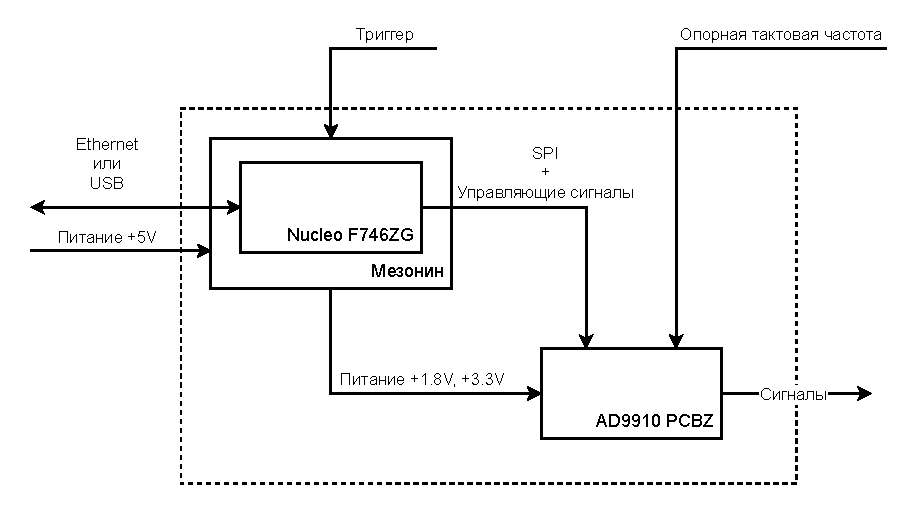
\includegraphics{data/system_architecture.drawio.pdf}
\caption{Общая схема устройства.}
\label{fig:system_architecture}
\end{figure}
\end{gostfigure}

Управление устройством осуществляется c ПК по USB или Ethernet, через виртуальный ком-порт в первом случае и через утилиту netcat во втором случае. Устройство предоставляет текстовый интерфейс, который включает в себя команды добавления сигналов в очередь, очистки очереди, запуска и остановки воспроизведения из очереди.

\pagebreak

Триггер может предоставляться как внешним устройством, так и самим микроконтроллером: на мезонинной плате предусмотрена перемычка, которая позволяет выбирать внешний либо внутренний источник. Частота следования триггеров может варьироваться в разумных пределах; внутренний источник сконфигурирован под стробирующий сигнал с частотой 25 Гц.

Ниже представлено схематичное изображение процесса подачи сигналов, схожее с тем, что можно было бы увидеть на осциллоскопе:

%
% Схематичное изображение процесса работы
%
\begin{gostfigure}
\begin{figure}[H]
\centering
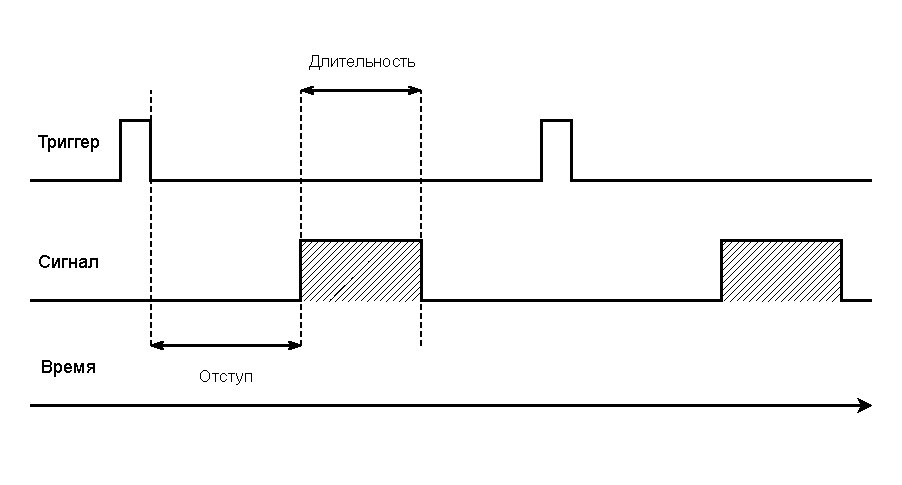
\includegraphics{data/timing_diagram.drawio.pdf}
\caption{Подача сигналов.}
\label{fig:timing_diagram}
\end{figure}
\end{gostfigure}

\subsection{Выбор инструментов}

Прошивка для микроконтроллера написана на языке программирования C, с использованием преимущественно свободных инструментов с открытым исходным кодом.

В качестве компилятора C использован gcc для ARM; все используемые в проекте библиотеки нацелены именно на этот компилятор, что и послужило главной причиной для его выбора. Возможной альтернативой является компилятор clang в составе проекта LLVM, но не проверялось, сможет ли он без ошибок собрать все задействованные библиотеки, в особенности STM32 HAL, который может содержать специфичный для gcc код.

В качестве системы сборки использован GNU Make. Задача Make состоит в запуске команд сборки, также называемых правилами, для каждого файла с исходным кодом. Главное преимущество от использования Make по сравнению с, например, скриптом сборки для интерпретатора командной строки, будь это bash или что-нибудь другое, заключается в возможности параллельной сборки, когда не зависящие друг от друга файлы с исходным кодом собираются параллельно, что позволяет существенно ускорить полную сборку проекта. Другим преимуществом является поддержка частичной сборки, когда повторно компилируются только файлы, изменившиеся с момента предыдущей сборки. Нужно отметить, что существуют и другие системы сборки, например CMake и ninja, которые обладают схожими возможностями, но часто сложнее в использовании.

В качестве IDE использована среда разработки VSCode, которая была выбрана преимущественно в связи с её популярностью и наличием расширения C/C++ IntelliSense, которое предоставляет быстрый поиск идентификаторов во всех файлах проекта и является незаменимым инструментом при изучении кода больших библиотек, таких как STM32 HAL. Нужно отметить, что, в отличие от самого VSCode, это расширение не является полностью свободным --- его исходный код закрыт. Другими IDE, которе бы подошли для разработки прошивки под ARM устройство, являются Qt Creator и CLion.

В качестве инструмента для загрузки собранной прошивки в микроконтроллер и отладки использован OpenOCD. Этот инструмент позволяет прошивать множество микроконтроллеров от разных производителей, а также выступает сервером отладки для gdb.

Наконец, в качестве отладчика использован gdb, который не имеет возможности самостоятельно взаимодействовать с отлаживаемым устройством и полагается на OpenOCD в качестве сервера.

\subsection{Использование STM32}

\subsubsection{Технические характеристики}

В данной работе используется отладочная макетная плата NUCLEO-F746ZG с процессором STM32F746ZG, системой питания, отладчиком ST-LINK и вспомогательной периферией (кнопки, порты, и т.д.). Характеристики микроконтроллера STM32F746ZG представлены ниже:

\begin{itemize}
	\item Ядро ARM Cortex-M7, оснащённое 4 КБ кэша инструкций и данных, работающее на частоте от 16 МГц до 216 МГц.
	\item Интерфейс SWD, позволяющий производить детальную отладку с компьютера, включая просмотр памяти и содержимого регистров процессора, а также добавление точек остановки на отдельные инструкции.
	\item 320 КБ внутренней оперативной памяти. Контроллер памяти в этом микроконтроллере предусматривает возможность добавления внешней оперативной памяти, но в рамках данного устройства эта возможность не используется.
	\item 1 МБ внутренней флэш-памяти. Эта память используется для хранения прошивки. Возможно добавление до 256 МБ внешней флэш-памяти при помощи интерфейса QSPI.
	\item Доступно вплоть до 168 GPIO, в зависимости от корпуса чипа и настроек интерфейсов.
	\item Множество периферийных интерфейсов, таких как SPI, UART, I2C, PWM, таймеры и др.
\end{itemize}

Более полные характеристики этого чипа можно найти в источнике \cite{STM32F746Datasheet}.

Макетная плата Nucleo примечательна следующим:

\begin{itemize}
	\item Встроенный модуль-отладчик, который позволяет питать плату от USB, производить отладку по протоколу ST-LINK v2, отвечает за процесс прошивки и предоставляет микроконтроллеру возможность отправлять и принимать данные с компьютера, выступая мостиком USB--UART.
	\item Ethernet-порт и микросхема PHY LAN8742A для подключения микроконтроллера к локальной сети.
	\item Три программируемых светодиода, которые можно использовать для индикации ошибок или событий.
	\item Гребенки контактов на нижней стороне платы и разъёмы на верхней стороне платы, которые выводят многие (но не все) GPIO с микроконтроллера.
\end{itemize}

Полный список характеристик этой отладочной платы можно найти в источнике \cite{NucleoDatasheet}.

\subsubsection{Компиляция прошивки}

В состав прошивки входят несколько ключевых компонентов:

\begin{itemize}
	\item Библиотека HAL для STM32F7xx, предоставляющая набор абстракций для работы с аппаратным обеспечением микроконтроллера. Распространяемый по лицензии BSD исходный код получен из официального репозитория и расположен в директории STM32CubeF7/ в рамках структуры файлов проекта.
	\item Ядро операционной системы FreeRTOS, реализующее многозадачность. Распространяемый по лицензии MIT исходный код получен из официального репозитория и расположен в директории FreeRTOS-Kernel/ в рамках структуры файлов проекта.
	\item Библиотека FreeRTOS-Plus-TCP с реализацией TCP/IP стека и драйвера для Ethernet-контроллера. Распространяемый по лицензии MIT исходный код получен из официального репозитория и расположен в директории FreeRTOS-Plus-TCP/ в рамках структуры файлов проекта.
	\item Набор дополнений к FreeRTOS, включая реализацию режима сна и аллокатор памяти с возможностью наращивания размера блоков. Построен с нуля или на основе кода других компонентов и расположен в директории freertos\_extras/ в рамках структуры файлов проекта.
	\item Библиотека picolibc в качестве стандартной библиотеки C, реализующей функции printf, scanf, strtod и др. В отличие от всех остальных компонентов, представлена в двоичной форме, а не в виде исходного кода. Расположена в файле libc.a в корневой директории в рамках структуры файлов проекта.
	\item Код приложения, связывающий все вышеперечисленные компоненты и реализующий:
	\begin{itemize}
		\item Инициализацию микроконтроллера.
		\item Текстовый пользовательский интерфейс.
		\item Алгоритмы управления синтезатором AD9910.
	\end{itemize}
\end{itemize}

Данный набор библиотек был получен не сразу. На ранних стадиях разработки использовался только HAL в сочетании с поставляющейся в комплекте с компилятором GCC стандартной библиотекой C newlib-nano, без использования операционной системы FreeRTOS.

Позднее, когда была реализована и проверена базовая логика управления синтезатором и настало время реализовать управление по Ethernet, было добавлено ядро FreeRTOS и библиотека FreeRTOS-Plus-TCP, и код приложения был адаптирован под использование предоставляемых FreeRTOS возможностей.

Наконец, библиотека newlib-nano была заменена библиотекой picolibc из-за неудовлетворительных характеристик предоставляемого в newlib-nano аллокатора памяти, а также отсутствия возможности переопределить функцию printf собственной версией, что требовалось для реализации перенаправления вывода при управлении по Ethernet. Библиотека picolibc не предоставляет аллокатор памяти, вместо этого был использован аллокатор heap5 в составе FreeRTOS, который был модифицирован для добавления поддержки функции realloc.

Процесс сборки прошивки происходит в два этапа: сборка отдельных файлов с исходным кодом (единиц трансляции) в объектные файлы, затем компоновка всех объектных файлов в итоговый бинарный файл с использованием использованием специфичного для микроконтроллера компоновочного скрипта.

Ниже представлен фрагмент файла Makefile, отвечающий за флаги компилятора при сборке и компоновке:

\lstset{
	language=c,
	basicstyle=\scriptsize\ttfamily,
	numbers=left,
	stepnumber=1,
	showstringspaces=false,
	tabsize=4,
	breaklines=true,
	breakatwhitespace=false,
	xleftmargin=.1\textwidth, xrightmargin=.1\textwidth,
	belowskip=1em, aboveskip=1em
}
\begin{lstlisting}
MCU_FLAGS = -mcpu=cortex-m7 -mfpu=fpv4-sp-d16 -mfloat-abi=hard

CC	 = arm-none-eabi-gcc
FLAGS	 = $(MCU_FLAGS) $(DEFINES) $(INCLUDE) -g -c -O2 -Wall -Wextra
LFLAGS	 = $(MCU_FLAGS) -T $(LDSCRIPT) -Wl,--print-memory-usage -Wl,--gc-sections -Wl,-Map=firmware.map,--cref -nostdlib
\end{lstlisting}

Здесь указывается тип процессора, под который требуется генерировать код, а также обозначается наличие аппаратного FPU одинарной точности. Помимо указания типа процессора, использован флаг {\footnotesize\ttfamily{``-g''}} для добавления минимальной отладочной информации и {\footnotesize\ttfamily{``-O2''}} для использования среднего уровня оптимизаций, а также включен набор предупреждений {\footnotesize\ttfamily{``-Wall -Wextra''}} о потенциальных ошибках в коде. Помимо этого, в переменной DEFINES передаётся набор директив препроцессора, необходимых для сборки HAL именно под чип STM32F746, а в переменной INCLUDE передаётся набор директорий для поиска заголовочных файлов.

Ещё один важный флаг компилятора указывается непосредственно в правиле для сборки отдельных файлов с кодом. Данное правило представлено ниже:

\lstset{
	language=c,
	basicstyle=\scriptsize\ttfamily,
	numbers=left,
	stepnumber=1,
	showstringspaces=false,
	tabsize=4,
	breaklines=true,
	breakatwhitespace=false,
	xleftmargin=.1\textwidth, xrightmargin=.1\textwidth,
	belowskip=1em, aboveskip=1em
}
\begin{lstlisting}
%.o: %.c
	@echo " [CC]" $<
	@$(CC) $(FLAGS) -flto -o $@ $<
\end{lstlisting}

Добавляемый здесь флаг {\footnotesize\ttfamily{``-flto''}} включает полнопрограммную оптимизацию, что приводит к заметному уменьшению размеров программы из-за удаления недостижимого кода.

При компоновке, для предотвращения включения в сборку поставляемой с компилятором стандартной библиотеки указывается флаг {\footnotesize\ttfamily{``-nostdlib''}}, а флагом {\footnotesize\ttfamily{``\verb!-Wl,-Map=firmware.map,--cref!''}} включается генерация детального отчёта о источнике каждой функции в итоговом файле, а также добавляется флаг {\footnotesize\ttfamily{``\verb!-Wl,--gc-sections!''}} для удаления незадействованного кода. Помимо этого, добавляется флаг {\footnotesize\ttfamily{``\verb!--Wl,--print-memory-usage!''}} для вывода объёма занятой флеш-памяти и объёма зарезервированной под статические переменные оперативной памяти, в виде короткого отчёта следующего вида по завершении компоновки:

\lstset{
	language=c,
	basicstyle=\scriptsize\ttfamily,
	numbers=left,
	stepnumber=1,
	showstringspaces=false,
	tabsize=4,
	breaklines=true,
	breakatwhitespace=false,
	xleftmargin=.1\textwidth, xrightmargin=.1\textwidth,
	belowskip=1em, aboveskip=1em
}
\begin{lstlisting}
Memory region         Used Size  Region Size  %age Used
             RAM:      100784 B       320 KB     30.76%
           FLASH:      175956 B         1 MB     16.78%
\end{lstlisting}

Размер и адрес регионов FLASH и RAM определён в компоновочном скрипте, путь к которому передан аргументом после флага {\footnotesize\ttfamily{``-T''}}. Помимо размеров памяти, компоновочный скрипт определяет порядок следования различных секций в памяти и предоставляет некоторые адреса в виде переменных, которые доступны в программном коде на C. В частности, компоновочный скрипт предоставляет адреса начала и конца кучи, что используется для инициализации аллокатора.

Ниже представлена таблица секций в порядке их следования в памяти:

% %%%%%%%%%%%%%%%%%%%%%%%
% Таблица секций в памяти
% %%%%%%%%%%%%%%%%%%%%%%%
\begin{table}[H]
\centering
\caption{Секции в памяти}
\label{tab:memory_sections}
\begin{tabular}{|c|c|p{8cm}|}
\hline 
\textbf{Название} & \textbf{Регион} & \textbf{Пояснение} \\ 
\hline 
.isr\_vector & FLASH & Таблица векторов прерываний \\ 
\hline
.text & FLASH & Исполняемый код \\ 
\hline
.rodata & FLASH & Константы \\ 
\hline
.data & FLASH, затем RAM & Переменные и локальные статические переменные, инициализированные ненулевым значением \\ 
\hline
.bss & RAM & Переменные и локальные статические переменные, инициализированные нулевым значением \\ 
\hline
\end{tabular} 
\end{table}

Изначально, использовался компоновочный скрипт из состава HAL, но в процессе интеграции FreeRTOS-Plus-TCP потребовалось внести в него изменения, в связи с чем была сделана копия вне директории HAL. Изменение заключалось в размещении входной секции first\_data в начале выходной секции data, что требуется драйвером Ethernet контроллера в составе FreeRTOS-Plus-TCP для расположения статически выделенных буферов в первых 64 КБ оперативной памяти.

Результатом компоновки является ELF файл с отладочной информацией, который можно использовать для прошивки микроконтроллера при помощи OpenOCD, что выполняется следующей целью в Makefile:

\lstset{
	language=make,
	basicstyle=\scriptsize\ttfamily,
	numbers=left,
	stepnumber=1,
	showstringspaces=false,
	tabsize=4,
	breaklines=true,
	breakatwhitespace=false,
	xleftmargin=.1\textwidth, xrightmargin=.1\textwidth,
	belowskip=1em, aboveskip=1em
}
\begin{lstlisting}
flash: firmware.elf
	openocd -f board/st_nucleo_f7.cfg -c "reset_config connect_assert_srst" -c "program firmware.elf verify reset exit"
\end{lstlisting}

При прошивке, во флеш-память микроконтроллера записываются исключительно код и данные, отладочная информация не попадает в микроконтроллер; она используется только во время отладки при помощи GDB для трансляции адреса выполняемой в определённый момент инструкции в номер строки исходного кода и других возможностей, упрощающих отладку. 

Важно отметить, что при использовании LTO отладочная информация обладает сниженной достоверностью, поскольку некоторые функции могут перестать существовать в виде отдельных сущностей после оптимизации. Рекомендуется производить целенаправленную отладку с выключенными оптимизациями LTO и флагом {\footnotesize\ttfamily{``-ggdb3''}} для получения наиболее детальной отладочной информации.

% TODO: Глава про отладку с GDB

\subsubsection{Инициализация}

После подачи питания или сброса, почти все периферийные устройства микрокроконтроллера находятся в выключенном состоянии, и ARM ядро работает на сниженной тактовой частоте. Одна из первых задач состоит в том, чтобы настроить тактирование для работы микроконтроллера на полной тактовой частоте, затем сконфигурировать периферийные устройства, которые будут использоваться в дальнейшем.

Выполнение кода начинается с функции-обработчика прерывания сброса из состава HAL, адрес которой ARM ядро извлекает из второй записи в таблице векторов прерываний, расположенной в самом начале флеш-памяти. Предварительно, ARM ядро инициализирует указатель стека таким образом, чтобы он указывал на конец оперативной памяти, исходя из первой записи в таблице. Поскольку стек растёт назад, это предоставляет максимально возможный размер стека для стартового кода. В рамках функции {\footnotesize\ttfamily{``Reset\_Handler''}} происходит заполнение секции .bss нулями, копирование секции .data из флеш-памяти в оперативную память, и включение FPU, после чего управление передаётся функции {\footnotesize\ttfamily{``main''}} уже в составе кода приложения.

Первым делом, код приложения настраивает аллокатор памяти, создаёт первую задачу и запускает планировщик FreeRTOS. Таким образом, ядро FreeRTOS на самом деле стартует до завершения инициализации оборудования. Далее, уже в контексте первой задачи, происходит вызов функции {\footnotesize\ttfamily{``system\_init''}}, которая последовательно инициализирует тактирование, затем отдельные перифералы.

После запуска микроконтроллера, тактирование осуществляется напрямую от внутреннего низкоточного источника тактовой частоты HSI со скоростью 16 МГц. На плате Nucleo доступен высокоточный источник тактовой частоты со скоростью 8 МГц, поступающий с отладчика. Для достижения полной тактовой частоты в 216 МГц используется блок PLL, который может работать от опорного тактового сигнала с частотой 1--2 МГц. Тактирование конфигурируется таким образом, что разделённый на 8 тактовый сигнал HSE поступает в PLL и умножается на 432, затем делится на 2, что даёт тактовую частоту в 216 МГц.

\subsubsection{Интерфейс SPI}

SPI --- вид шины для последовательной передачи данных. Для коммуникации с одним устройством используется три линии: MOSI, MISO, SCK. На линии SCK находится тактовый сигнал устройства-мастера, MOSI передаёт данные от мастера к клиенту, а MISO, наоборот, от клиента к мастеру. За один такт передаётся один бит информации в одном направлении. Возможно добавление неограниченного количества устройств-клиентов, но на каждое потребуется по одной дополнительной линии выбора, которую обычно называют CS (Chip Select).

Зачастую, возможна полностью программная реализация SPI, но аппаратная реализация в STM32 обладает рядом преимуществ: она убирает необходимость программным образом разделять данные на отдельные биты и позволяет использовать DMA.

Проверить работоспособность SPI можно без использования дополнительных устройств: если соединить линии MOSI и MISO устройства-мастера, то оно будет посылать данные само себе. Линия SCK при этом остаётся не подключенной. В случае, если полученные данные отличаются от отправленных, можно сделать вывод о наличии проблем с работой SPI.

\subsubsection{Интерфейс UART}

UART --- вид шины для последовательной передачи данных, как и SPI, но главное отличие UART заключается в асинхронности. Передача данных осуществляется по двум линиям: TX (отправка) и RX (приём). Линия с тактовым сигналом отсутствует, вместо этого для обозначения начала и окончания данных используются стартовые и стоповые биты. Как правило, на одной шине UART никогда не размещается больше двух устройств. Для корректной передачи данных, оба устройства обязательно должны быть настроены на использование одинаковой скорости.

Микроконтроллеры STM32 реализуют USART --- расширенную версию UART, в которой возможна работа в синхронном режиме с использованием дополнительной линии для тактовой частоты. Когда синхронный режим не требуется, USART можно использовать как обычный UART.

Из нескольких присутствующих в микроконтроллере блоков USART, интерес представляет именно USART3, поскольку его вход и выход связан с отладчиком. В процессе инициализации, USART3 настраивается для работы со скоростью 115200 бит/секунду, с 8 битами данных в посылке и одним стоповым битом. Данная конфигурация широко известна как ``115200 8N1''. 

Для отправки сообщений на ПК используется передача в блокирующем режиме, когда ARM ядро в цикле ожидает завершения передачи одного байта перед тем, как отправить следующий.

Для получения команд с ПК используется режим DMA с прерыванием по переходу линии в состояние простоя. Предварительно, блок DMA настраивается под копирование значений из регистра приёма в буфер в оперативной памяти. Затем, по мере поступления посылок с ПК, блок USART3 создаёт DMA запросы и полученные байты сохраняются в оперативной памяти микроконтроллера без участия ARM ядра.

Если для ввода команды используется клавиатура и нажатия клавиш происходит медленно, то линия будет переходить в состояние простоя после каждого отдельного нажатия. Если же команда или набор команд были вставлены в окно терминальной программы из буфера обмена, то они будут получены непрерывной чередой посылок, и линия перейдёт в состояние простоя только после передачи последнего байта. И в том и в другом случае, переход линии в состояние простоя приведёт к остановке получения и срабатыванию прерывания.

В рамках функции-обработчика прерывания происходит:

\begin{itemize}
	\item Отправка копии полученных данных обратно на ПК, чтобы они отобразились в окне терминальной программы.
	\item Обработка стирания.
	\item Добавление вызова функции разбора в очередь отложенных задач, если последний полученный символ является переносом строки, и перезапуск процесса получения в обратном случае.
\end{itemize}

В рамках функции разбора происходит поиск отдельных разделённых переносами команд, каждая из которых передаётся интерпретатору команд, после чего происходит перезапуск процесса получения.

\subsubsection{Интерфейс Ethernet}

Ethernet является широко распространённым интерфейсом для подключения компьютеров к локальной сети и обладает существенно более высокой сложностью по сравнению с рассмотренными ранее интерфейсами.

В состав Ethernet контроллера входят два отдельных аппаратных блока: MAC и PHY. Блок PHY реализует физический уровень модели OSI и отвечает за кодирование и декодирование электрических сигналов в кабеле, а блок MAC реализует канальный уровень и отвечает за фильтрацию входящих фреймов, проверку и генерацию контрольных сумм, копирование полученных фреймов в оперативную память микроконтроллера в автономном режиме через собственный контроллер DMA, и некоторые другие возможности.

Использующийся в Ethernet сетях стек протоколов TCP/IP тоже обладает высокой сложностью, поэтому в данной работе используется FreeRTOS-Plus-TCP --- готовая реализация стека TCP/IP для операционной системы FreeRTOS, включающая  большой набор драйверов для встречаемых в разных микроконтроллерах комбинаций MAC и PHY.

Предоставляемый FreeRTOS-Plus-TCP набор функций для работы с сокетами концептуально похож на сокеты Беркли, несмотря на другие названия функций. Кроме API для работы с сокетами, разработчиком может быть реализован набор обратных вызовов, которые используются для оповещения приложения об установлении или разрыве соединения.

Почти вся конфигурация выполняется ещё до этапа компиляции, через заголовочный файл, где директивы препроцессора включают или отключают отдельные возможности и протоколы. Данный подход позволяет минимизировать объём занятой флеш-памяти, поскольку выключенные части кода не попадают в сборку. Во время исполнения, для запуска FreeRTOS-Plus-TCP должны быть указаны всего несколько начальных параметров:

\begin{itemize}
	\item MAC адрес.
	\item IP адрес.
	\item Маска подсети.
	\item Адрес шлюза.
	\item Адрес DNS сервера.
\end{itemize}

Если в конфигурации FreeRTOS-Plus-TCP включен DHCP клиент, данные параметры (за исключением MAC адреса) становятся резервными параметрами на тот случай, когда получение конфигурации по DHCP не удалось. Если же DHCP клиент выключен, то указанные параметры используются сразу.

В результате запуска FreeRTOS-Plus-TCP создаётся задача ``IP-task,'' внутри которой обрабатываются связанные с сетью события.

Далее, запускается задача с TCP сервером, который начинает прослушивать порт 80 и принимает входящие подключения. Для обслуживания каждого нового подключения создаётся отдельная задача, в которую параметром передаётся указатель на сокет принятого подключения. Внутри задачи обслуживания происходит настройка перенаправления вывода таким образом, чтобы все вызовы printf приводили к отправке сообщения в сокет а не в последовательный порт. Далее, в цикле происходит получение входящих байт в буфер приёма и поиск команд, разделённых символами переноса строки. Каждая команда передаётся интерпретатору команд. В случае разрыва подключения по инициативе клиента, задача удаляется.

\subsubsection{Интерпретатор команд}

Интерпретатор команд состоит из главной функции выбора и множества функций обработчиков. В функции выбора происходит извлечение первого слова команды, после чего оно последовательно сравнивается со всеми известными именами команд текстового интерфейса, и в случае совпадения происходит вызов соответствующего обработчика с полным текстом команды в качестве аргумента.

Если у команды нет аргументов, то обработчик не выполняет никаких действий с полученным тестом команды. Если же у команды есть аргументы, то обработчик считывает их в переменные. Количество аргументов проверяется и в случае нехватки аргументов обработчик выходит с сообщением об ошибке.

Почти все связанные с подачей сигналов команды поддерживают указание частоты и времени в наиболее удобных единицах: ns, us, ms, s для времени и Hz, kHz, MHz для частоты. В обработчиках все значения приводятся к нс и Гц, поскольку именно эти единицы наиболее удобны для работы учитывая разрешение таймеров микроконтроллера и синтезатора.

\subsubsection{Управление синтезатором}

Значительная часть логики, непосредственно реализующей различные режимы работы калибратора, реализована в секвенсоре --- компоненте, который отвечает за воспроизведение заданных последовательностей сигналов. В основе секвенсора лежит универсальная структура данных для описания сигналов, и динамический массив данных структур служит для представления последовательности сигналов с разными параметрами.

В структуре данных содержатся точки начала и завершения сигнала, представляющие отступ и длительность, значения трёх параметров сигнала для всех профилей, необязательный массив с последовательностью переключения профилей, а также необязательный образ оперативной памяти и параметры воспроизведения.

В самом секвенсоре выполняется несколько ключевых операций:

\begin{itemize}
	\item На основе структуры данных для описания сигналов и при помощи набора предоставляемых драйвером AD9910 функций, секвенсор изменяет хранящийся в памяти микроконтроллера снимок регистров синтезатора и выполняет перезапись регистров синтезатора этим снимком на стадии подготовки к подаче очередного сигнала.
	\item В зависимости от наличия какой-либо последовательности переключения профилей в структуре данных сигнала, DMA настраивается под использование предоставленного в структуре данных буфера в качестве источника значения профилей, либо под использование буфера по умолчанию, где находится значение для включения одного активного профиля в момент начала сигнала.
	\item Если присутствует последовательность переключения профилей, таймер модуляции настраивается на отсчёт длительности одного элемента последовательности. Если последовательности нет, таймер модуляции не будет запущен и создаст только один DMA запрос, в результате сброса в момент начала сигнала.
	\item В случае сигнала с нулевым отступом, включается альтернативный механизм связывания таймера сигнала и таймера модуляции. 
	\item В регистры сравнения таймера сигнала записываются точки начала и завершения сигнала.
\end{itemize}

Некоторые части реализации различных режимов работы расположены в обработчиках отдельных команд в текстовом интерфейсе, где происходит заполнение используемой секвенсором структуры данных. Там выполняются те действия, которые желательно сделать заранее, например построение образов оперативной памяти AD9910, или построение буферов модуляции профилями, если данная возможность используется. Главной целью выполнения подобных задач заранее является сведение к минимуму затрат времени на реконфигурацию между триггерами путём сужения круга требуемых действий исключительно до записи заранее подготовленных значений в регистры синтезатора.

\subsection{Использование AD9910}

Цифровой синтезатор сигналов (DDS) AD9910 представлен в исполнении производителя на отладочной плате AD9910 PCBZ. Данная плата предусматривает управление при помощи внешнего микроконтроллера через выведенные на контактные гребенки входы и выходы, либо с ПК при помощи интерфейса USB, который реализован неизвестным микроконтроллером на плате.

Ниже представлены некоторые ключевые характеристики AD9910:

\begin{itemize}
	\item Максимальная внутренняя частота: 1 ГГц.
	\item Разрядность ЦАП: 14 бит.
	\item Восемь профилей частоты, амплитуды и начальной фазы сигнала, между которыми возможно быстрое переключение.
	\item Параллельный порт для быстрого изменения одного из параметров сигнала.
	\item Внутренняя оперативная память для сложных сигналов.
\end{itemize}

% TODO: Объяснить в теоретической части, что чем выше тактовая частота DDS, тем больше точность аппроксимации
Источником тактовой частоты для синтезатора может выступать кварцевый резонатор на плате или внешний генератор. В случае использования внешнего генератора, есть три способа получения максимальной внутренней частоты: AD9910 может работать на прямую от поступающей от внешнего источника частоты, либо может делить её на два через встроенный делитель или умножать на число от 12 до 127 при помощи встроенного PLL (Блока ФАПЧ); это позволяет использовать внешние частоты, равные 1 ГГц, 2 ГГц или $\frac{1}{x}$ ГГц, где $12 \leq x \leq 127$ и $x$ является целым. Для первичной проверки работоспособности синтезатора использовалась внешняя частота равная 200 МГц и AD9910 работал на сниженной скорости.

В режиме управления с ПК, синтезатор подключается по USB, и используя утилиту от производителя (представлена на рисунке \ref{fig:ad9910_evaluation_software}) можно управлять всеми его настройками, видя при этом изменения в содержимом регистров. Это крайне полезный инструмент для ознакомления с устройством.

\begin{gostfigure}
\begin{figure}[H]
\centering
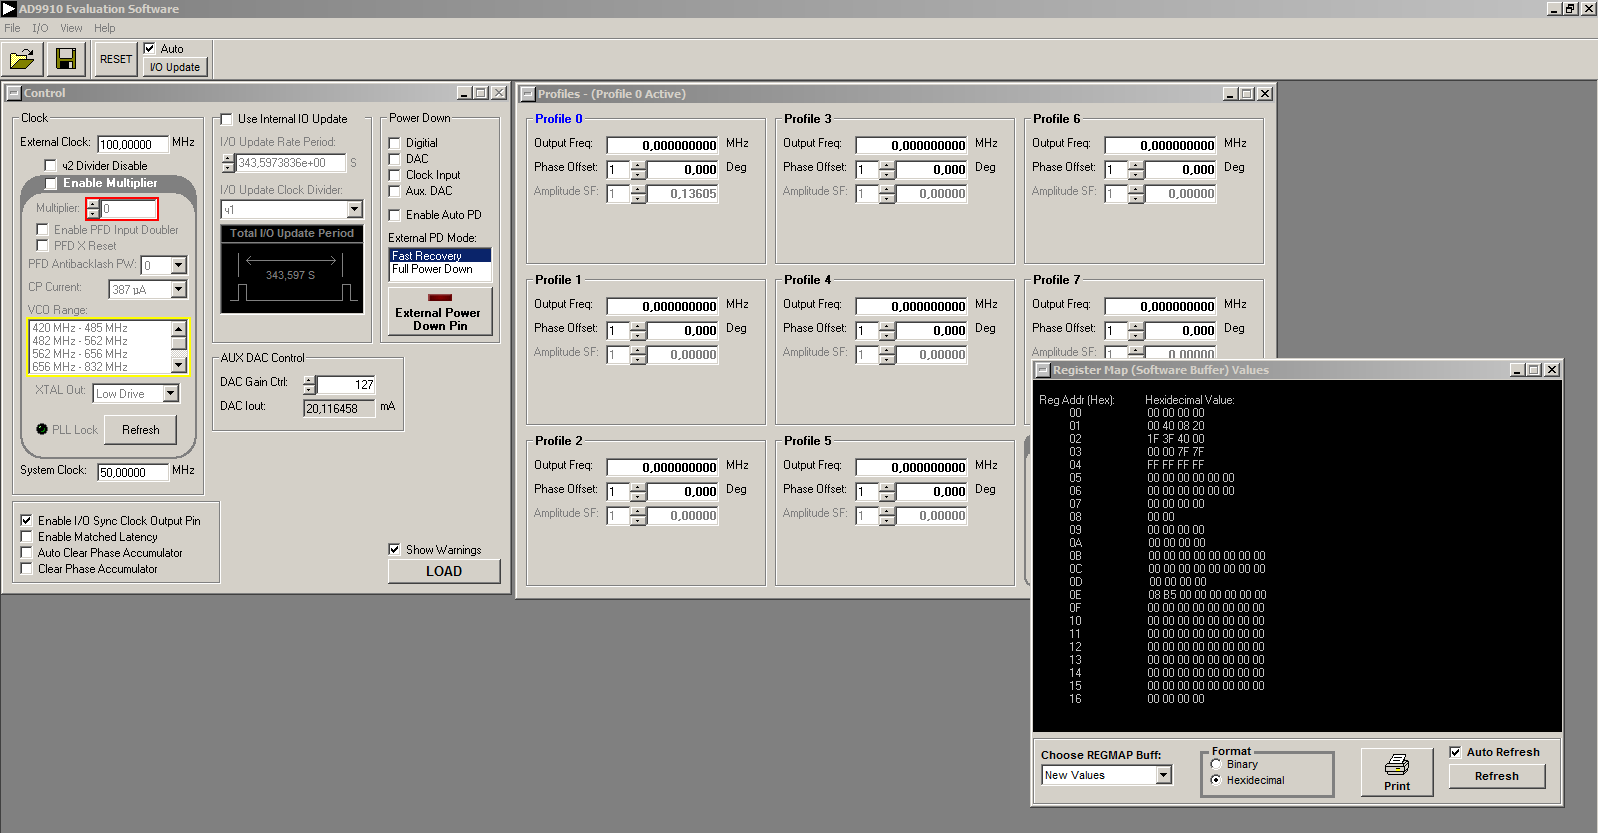
\includegraphics[scale=.25]{data/ad9910_evaluation_software.png}
\caption{Утилита управления синтезатором AD9910 с ПК.}
\label{fig:ad9910_evaluation_software}
\end{figure}
\end{gostfigure}

Всего синтезатор имеет 23 регистра с различной шириной, от 2 байт до 8 байт. В большинстве случаев, один бит регистра отвечает за включение/выключение определённой функции синтезатора, но есть некоторые регистры, которые отведены под хранение числовых значений, например регистры 15--22 используются для хранения восьми профилей генерируемой частоты. Полное описание полей регистров чипа AD9910 можно найти в источнике \cite{AD9910Datasheet}.

Расположенный на плате синтезатора микроконтроллер не подходит для решения поставленной задачи по двум причинам: во-первых, у него нет интерфейса Ethernet, а это является одним из требований к устройству. Во-вторых, исходные коды его существующей прошивки нигде не доступны. Поэтому встроенный микроконтроллер был отключен перестановкой перемычек на плате.

Управление внешним микроконтроллером осуществляется при помощи множества выделенных под отдельные функции синтезатора управляющих сигналов, а также SPI для доступа к регистрам.

Используемые для SPI входы и выходы представлены в таблице \ref{tab:spi_pins}:

% %%%%%%%%%%%%%%%%%%%%%%%%%%%%%%%%%%%%%%%%%%%%%%%%%%%%
% Таблица используемых для SPI входов и выходов AD9910
% %%%%%%%%%%%%%%%%%%%%%%%%%%%%%%%%%%%%%%%%%%%%%%%%%%%%
\begin{table}[H]
\centering
\caption{Используемые для SPI входы и выходы AD9910}
\label{tab:spi_pins}
\begin{tabular}{|p{4cm}|p{8cm}|}
\hline 
\textbf{Название} & \textbf{Пояснение} \\ 
\hline 
CSB & Низкий уровень на этом входе активирует порт SPI синтезатора \\ 
\hline
SCLK & Тактовый сигнал SPI подаваемый устройством-мастером \\
\hline
SDO & Выход SPI для отправки данных устройству-мастеру \\
\hline
SDIO & Вход SPI для получения данных от устройства-мастера, или вход и выход одновременно, в зависимости от выбранного режима SPI \\
\hline 
IO\_RESET & Высокий уровень на этом входе отменяет текущую транзакцию \\
\hline
\end{tabular} 
\end{table}

В рамках одной SPI транзакции синтезатору сначала отправляется инструкция размером в один байт, где старший бит выбирает между режимом записи и режимом чтения, а пять младших битов определяют номер интересующего регистра. В режиме записи должны последовать {\em n} байт данных, где {\em n} --- ширина регистра, а в режиме чтения, наоборот, должно быть считано {\em n} байт данных.

Значения, записанные в регистры синтезатора, вступают в силу не сразу. Изначально они находятся в буфере ввода-вывода, и чтобы скопировать их в действующие регистры, нужно подать короткий сигнал высокого уровня на вход IO\_UPDATE, что далее по тексту называется ``Выполнить IO\_UPDATE.'' Перенос значений в действующие регистры также произойдёт в результате изменения состояния входов профилей, когда происходит выбор профиля, отличного от выбранного ранее.

\subsubsection{Первый запуск}

Для начального запуска синтезатора под управлением микроконтроллера был использован подход с записью всех регистров эталонными значениями: благодаря утилите производителя было известно, какое в точности содержимое должно быть в каждом регистре синтезатора для получения непрерывного сигнала на некоторой частоте. Так как внутреннее состояние синтезатора представлено только его регистрами, можно перезаписать содержимое всех регистров этими заранее известными значениями, и, при прочих равных условиях, синтезатор должен начать генерировать сигнал на выходе. Технически, содержимое оперативной памяти тоже является внутренним состоянием синтезатора, но на данном этапе оперативная память не используется.

Здесь встретилась первая значительная проблема: изначально синтезатор совершенно не хотел взаимодействовать с микроконтроллером, не отвечая на запросы по шине SPI и не выдавая никаких сигналов даже после записи всех необходимых регистров вслепую. Первое предположение о причине проблемы заключалось в том, что на микроконтроллере как-то неправильно настроена шина SPI. Было опробовано множество различных комбинаций скоростей, полярностей и фаз, безрезультатно. Плата синтезатора несколько раз конфигурировалась обратно в режим управления с ПК, что подразумевает перестановку нескольких перемычек, чтобы убедиться, что синтезатор не выработал какую-то поломку.

Далее, управляющие сигналы на плате синтезатора были тщательно изучены при помощи осциллоскопа, с целью найти какие-нибудь различия при работе в режиме управления с ПК и в режиме управления с микроконтроллера. Прослушивание шины SPI при отправке команд из утилиты производителя позволило определить гарантированно работоспособные параметры SPI --- вторым предположением было, что продолжительность либо порядок управляющих сигналов, которые поступают с микроконтроллера, не соответствует спецификациям AD9910. Все задержки были приведены к абсолютно безупречному виду на осциллоскопе, но синтезатор всё равно не работал.

Единственной зацепкой, которую удалось найти, было следующее: когда плата сконфигурирована под управление микроконтроллером, исчезает сигнал в гнезде SYNC\_CLK, который иначе присутствует после первого запуска утилиты производителя и составляет ¼ частоты внешнего источника. Это привело к мысли, что микроконтроллер пытаемся отправлять AD9910 команды, когда последний находится в состоянии, в котором он не готов их получать. Исходя из этого возникло третье предположение: проблема имеет исключительно электрический характер; удаление перемычек, которые включают режим управления с ПК, может менять электрические характеристики на плате, например, некоторые ножки чипа AD9910 могут оказаться в неопределенном состоянии, когда раньше они были подтянуты к низкому или высокому уровню.

В конце концов это и оказалось истинным источником проблемы --- входы MASTER\_RESET и EXT\_PWR\_DWN, которые отвечают за общий сброс чипа и переход в спящий режим соответственно, переходили в неопределенное состояние. Этого было достаточно, чтобы чип не запускался. Достаточно было подтянуть два этих сигнала к нулю, чтобы синтезатор начал надежно запускаться, выдавая ожидаемый сигнал в SYNC\_CLK.

После этих действий чип действительно начал реагировать на команды, поступающие от микроконтроллера. Получилось понаблюдать за изменениями, происходящими от переключения отдельных битов в регистрах. Поставив перемычки между GND и входами P\_0, P\_1 и P\_2, которые отвечают за выбор профиля, чтобы привести их из неопределённого состояния к низкому уровню и принудительно выбрать нулевой профиль, и записав заранее заготовленные значения в регистры профилей, мы смогли, наконец, получить сигнал на выходе синтезатора.

Далее удалось переключить синтезатор в трёхпроводной режим SPI, что дало возможность считывать содержимое регистров. Теоретически, использование двухпроводного режима тоже возможно, но используемый микроконтроллер имеет некоторые проблемы с размером считываемых данных в этом режиме, поэтому трёхпроводной режим предпочтителен.

\subsubsection{Формирование непрерывных сигналов}

% Реализовано в:
% - https://github.com/AXKuhta/stm32_ad9910/commit/272f2d1457d6abef2580f479caacd4918fd27638
% - https://github.com/AXKuhta/stm32_ad9910/commit/0c8fbba4f038878d401e76cec10e339cd68cf210
Переход от записи полностью фиксированных значений в регистры к программному изменению основных параметров сигнала стал следующим шагом.

На генерируемый синтезатором сигнал влияют три основных параметра:

\begin{table}[H]
\centering
\caption{Параметры сигнала в AD9910}
\label{tab:signal_parameters}
\begin{tabular}{|p{4cm}|p{8cm}|}
\hline 
\textbf{Название} & \textbf{Пояснение} \\ 
\hline 
$FTW$ & 32-х битное значение частоты. \\ 
\hline
$POW$ & 16-ти битное значение сдвига фазы. \\
\hline
$ASF$ & 14-ти битное значение амплитуды. \\
\hline
\end{tabular} 
\end{table}

За выбор источника $FTW$, $POW$ и $ASF$ отвечает коммутатор шин, прямого контроля над которым нет и который автоматически выбирает один источник из набора активных источников на основе определённых аппаратно приоритетов. В конфигурации по умолчанию, частота и фаза берутся из регистров профилей, а амплитуда берётся из общего вторичного регистра. Чтобы включить индивидуальную амплитуду для каждого профиля, необходимо включить бит Enable Amplitude Scale from Single Tone Profiles, который выключен по умолчанию.

Ниже представлена структура полей одного профиля:

%
% Структура полей в регистрах профилей.
%
\begin{gostfigure}
\begin{figure}[H]
\centering
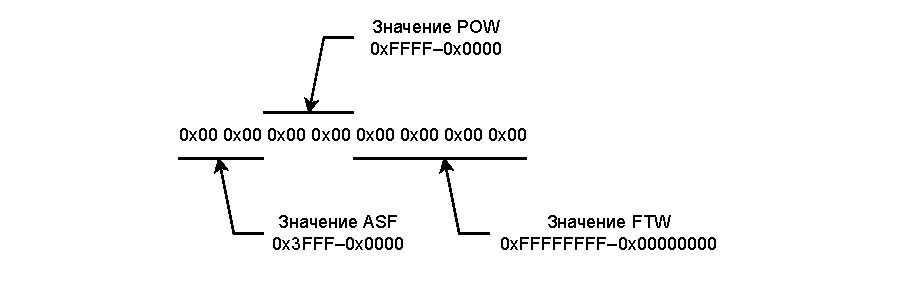
\includegraphics{data/single_tone_profile_register_layout.drawio.pdf}
\caption{Структура полей в регистрах профилей.}
\label{fig:single_tone_profile_register_layout}
\end{figure}
\end{gostfigure}

Для подачи сигналов на некоторой произвольной частоте необходимо вычислить значение $FTW$ по формуле $a\frac{2^{32}}{b}$, где $a$ --- требуемая частота в Гц, а $b$ --- тактовая частота синтезатора в Гц, затем вставить это значение в один из профилей. Также потребуется выставить значение амплитуды.

Был реализован набор функций для изменения частоты и амплитуды профилей в хранимой микроконтроллером копии регистров синтезатора. Для активации изменений все регистры синтезатора перезаписываются обновлённым снимком регистров, после чего выполняется IO\_UPDATE.

Это стало основой для команды выдачи непрерывного сигнала на одной частоте {\footnotesize\ttfamily{test\_tone [freq] [unit]}}, которая была позднее реализована в текстовом интерфейсе. Данный режим полезен при изучении качества генерируемого сигнала при помощи анализатора спектра, где, как правило, требуются непрерывный сигнал. Анализаторы спектра могут показать наличие шумов и гармоник, которые неизбежно будут присутствовать в генерируемом DDS сигнале. Также режим фиксированного тона можно использовать, чтобы убедиться, что PLL синтезатора установился на требуемой частоте. Между двумя сигналами, первый из которых создаётся синтезатором, а второй создаётся другим генератором, работающим от того же источника опорной тактовой частоты, не должно наблюдаться смещения волн относительно друг друга при просмотре на осциллоскопе. Здесь нужно иметь ввиду, что должна быть выставлена частота, которую можно получить в результате суммирования одного или более частных от деления внутренней частоты синтезатора на степень двойки, поскольку DDS могут генерировать только такие частоты с абсолютной точностью.

Говоря про PLL, следующим шагом после получения сигнала из синтезатора стало задействование блока PLL, чтобы начать использовать синтезатор на полной скорости путём умножения опорной частоты.

Блок PLL в AD9910 состоит из нескольких регулируемых напряжением источников частоты (VCO), предназначенных для работы в разных диапазонах частот. Из всех VCO выбирается тот, в диапазон которого попадает требуемая внутренняя частота синтезатора. Так как мы хотим использовать синтезатор на его максимальной тактовой частоте, мы выбираем самый быстрый VCO. Принцип работы ФАПЧ (PLL) заключается в измерении расхождения между частотой VCO, разделённой на некоторое число, и опорной частотой. Расхождение используется, чтобы регулировать напряжение VCO для минимизации ошибки в частоте, и в результате обратной связи VCO достаточно быстро устанавливается на требуемой частоте. В целом, VCO в блоке PLL может работать и без опорной частоты, но тогда внутренняя частота синтезатора определена лишь примерно. Если не рассматривать PLL в деталях, то проще думать о нём, как о некотором компоненте синтезатора, который может осуществлять умножение опорной тактовой частоты на множители в диапазоне $12\times$--$127\times$. Выбор множителя осуществляется изменением полей в регистрах, после чего PLL включается установкой соответствующего бита.

Здесь была встречена следующая проблема: при использовании PLL, сигнал на выходе синтезатора приобретал крайне нестабильный характер. На выходе PLL\_LOCK, который должен сигнализировать, что PLL установился на нужной частоте, сохранялся низкий уровень. Причина заключалась в том, что для использования PLL требовалось установить на плату синтезатора несколько дополнительных компонентов, которые образуют низкочастотный фильтр, который сглаживает сигнал ошибки и необходим для правильной работы PLL. Что интересно, обязательность этих компонентов была явным образом обозначена в инструкции к отладочной плате, но не в даташите от AD9910. Производитель предоставляет построенный в виде таблицы для MS Excel инструмент (PLL Loop Filter Tool), который позволяет вычислить наиболее подходящие для используемой опорной частоты номиналы компонентов фильтра, что и было сделано. Руководствуясь полученными в результате вычислений значениями, на плату синтезатора были установлены компоненты,сконфигурировавшие её под опорную частоту, составляющую примерно 20 МГц. Это помогло разрешить проблему --- на выходе PLL\_LOCK начал возникать высокий уровень, и сигнал на выходе синтезатора стал стабильным. Данный момент был важен, так как синтезатор впервые заработал на своей полной внутренней частоте в 1 ГГц.

Важно отметить, что только блоки, непосредственно связанные с генерацией сигнала работают на полной тактовой частоте. В их набор входит аккумулятор фазы, конвертер угла в амплитуду и скалер амплитуды, а также ЦАП. Все остальные части синтезатора, такие как интерфейсы и внутренние источники параметров сигнала, работают на четверти внутренней тактовой частоты.

Управление состоянием входов профилей на синтезаторе стало следующей задачей. Возможность быстро изменять все три параметра сигнала посредством профилей позволяет реализовать модуляцию. Например, можно использовать два профиля с одинаковой частотой и амплитудой, но различающейся на 180° фазой, чтобы реализовать модуляцию BPSK. Были убраны поставленные ранее перемычки и входы P\_0, P\_1 и P\_2 были подключены к микроконтроллеру

\subsubsection{Формирование коротких импульсов}

Наконец, мы подошли к самой главной проблеме использования синтезатора: формирование импульсов вместо непрерывных сигналов. Для этого требуется реализовать прекращение и возобновление подачи сигнала, и существует несколько разных способов сделать это на AD9910. Даташит не рассматривает конкретный сценарий использования с формированием импульсов и, следовательно, не содержит информации о том, какой из подходов лучше.

Первый подход состоит в использовании нулевой амплитуды в одном из профилей. Включение такого профиля приведёт к тому, что независимо от остального состояния синтезатора, после блока масштабирования по внутренней шине данных на ЦАП будут поступать только нули, и сигнала на выходе не будет. Недостаток этого метода заключается в том, что один профиль потребуется навсегда зарезервировать как ``парковочный'' профиль, и для модуляции останутся доступны только семь профилей, что сделает невозможным создание некоторых видов модуляции, например 8-PSK, хотя, как обнаружилась позднее, модуляция 8-PSK при помощи профилей всё равно невозможна из-за другой проблемы, которую не получилось решить.

Второй подход заключается в использовании блока OSK в синтезаторе, который предназначен для управления амплитудой и может достичь схожего эффекта с применением нулевой амплитуды к сигналу в зависимости от уровня на выделенном входе OSK. Недостаток OSK заключается в том, что он имеет наибольший возможный приоритет в качестве источника амплитуды в синтезаторе, и когда он включен, пропадает возможность использовать амплитуду из профилей или оперативной памяти, что очень критично. Из-за этого было решено вообще не использовать OSK и не подводить его управляющий вход к микроконтроллеру.

Третий подход заключается в использовании статического сброса накопителя фазы в сочетании с режимом вывода синусоиды --- двух возможностей, которые доступны через регистры синтезатора. Как и в предыдущем способе, это приведёт к поступлению исключительно нулей по внутренней шине данных на ЦАП и отсутствию сигнала на выходе. Главная проблема с этим подходом состоит в том, что потребуется больше времени, чем с переключением профилей, так как необходимо произвести запись одного регистра по SPI, затем выполнить IO\_UPDATE.

Четвертый подход заключается в использовании входа EXT\_PWR\_DOWN для отправки синтезатора в режим пониженного энергопотребления с быстрым восстановлением, когда все блоки синтезатора кроме PLL отключаются. Здесь не имеет значения состояние внутренней шины данных, так как ЦАП отключается по-настоящему. Несмотря на то, что таким образом действительно можно прекратить подачу сигналов, данный метод не подойдёт для наших целей, так как он также отключает порт SPI и убирает возможность изменять регистры синтезатора в промежутке между импульсами.

% Реализовано в:
% - https://github.com/AXKuhta/stm32_ad9910/commit/2e487a1fa9ddbbce861b1afd3613c8091fd185eb
В итоге был выбран первый способ, когда нулевой профиль зарезервирован под прекращение подачи сигнала и режим ожидания триггера. Для начала подачи сигнала происходит переключение на другой профиль с ненулевой амплитудой. В изначальной реализации переключение профиля осуществлялось из контекста прерывания на микроконтроллере, с достаточно большим разбросом по времени. Позднее, для установки уровней на входах профилей был задействован DMA, что позволило уменьшить разброс.

У этого подхода присутствует одна проблема: непредсказуемая начальная фаза сигнала. Включение профиля с нулевой амплитудой и нулевой частотой уберёт сигнал с выхода и остановит изменение значения в накопителе фазы, но накопитель не будет сброшен, и в этом кроется проблема: в момент начала следующего импульса старое значение фазы приведёт к началу сигнала со значения синуса в произвольной точке, а не в нуле, что будет выглядеть на осциллоскопе как резкий прыжок или резкий провал, после которого начинает следовать нормальная синусоидальная волна. Наличие таких разрывов в сигнале нежелательно, но в целом терпимо. Из непредсказуемой начальной фазы также следует непредсказуемость фазы во всех остальных точках сигнала. Иными словами, положение пиков в синусоидальной волне на протяжении всего сигнала будет различаться между запусками, что тоже нежелательно, но терпимо, т.к. не препятствует использованию устройства для снятия АЧХ.

На рисунке ниже представлено наглядное изображение проблемы: слева изображено начало синусоидального сигнала с нулевой фазой, а справа начало синусоидального сигнала со случайной фазой.

%
% Нулевая начальная фаза и случайная начальная фаза.
%
\begin{gostfigure}
\begin{figure}[H]
\centering
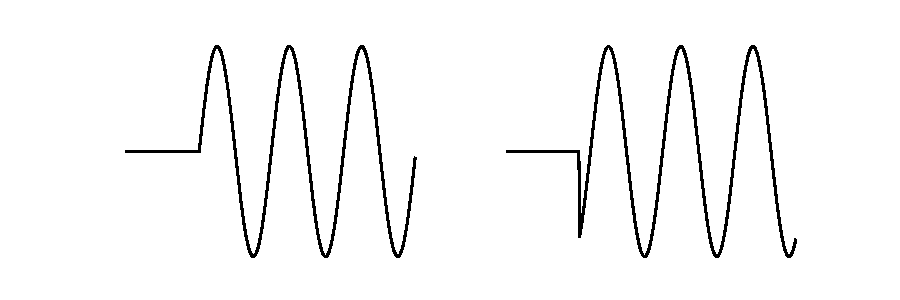
\includegraphics{data/random_start_phase.pdf}
\caption{Нулевая начальная фаза и случайная начальная фаза.}
\label{fig:random_start_phase}
\end{figure}
\end{gostfigure}

% https://tex.stackexchange.com/questions/168430/xelatex-polyglossia-hyphenation
Тем не менее, проблему с непредсказуемой начальной фазой можно исправить. Как уже упоминалось ранее, у синтезатора присутствует возможность статического сброса накопителя фазы, когда его значение удерживается на нуле. На самом деле, существует два способа сбросить накопленную фазу: статический сброс, который переключается битом \textenglish{Clear phase accumulator} в регистрах, и сброс при переключении профилей, который переключается битом Autoclear phase accumulator. В случае со сбросом по переключению профиля механизм работы достаточно понятен: при каждом изменении состояния входов профилей, фаза сбрасывается. Для сигналов, в которых отсутствует модуляция при помощи профилей, можно без опаски использовать этот способ сброса фазы, так как профиль будет переключаться только в начале и в конце сигнала, и никогда не будет переключаться посередине. Если же используется модуляция при помощи профилей, то использование Autoclear phase accumulator приведёт к сбросу фазы в моменты смены элементов кода, создавая разрывы в сигнале, а в случае с PSK модуляцией вообще затруднит использование, т.к. этот вид модуляции полагается на сдвиг фазы относительно предыдущего значения, а не переход на абсолютное значение. В этом случае лучше подойдёт статический сброс фазы, принцип работы которого несколько сложнее: при включении бита Clear phase accumulator, накопитель фазы принудительно удерживается в сброшенном состоянии, т.е. всегда равен нулю и не увеличивается.

Чтобы начать подачу сигнала из этого состояния, нужно выключить статический сброс до начала подачи следующего сигнала и вызвать применение изменений, выполнив IO\_UPDATE. После выключения статического сброса, если выбран профиль с нулевой частотой, то значение накопителя не начнёт увеличиваться и по шине данных на ЦАП продолжат поступать нули. Затем, когда будет включен профиль с ненулевой частотой, значение накопителя фазы начнёт расти с нуля и на выходе получится сигнал с предсказуемой начальной фазой. Здесь стоит вспомнить, что применение изменений в регистрах происходит не только от IO\_UPDATE, но и от переключения профилей, так что применение IO\_UPDATE после отключения статического сброса необязательно, т.к. изменения всё равно будут применены в момент схода с парковочного профиля.

Ниже представлена диаграмма, на которой изображена выбранная схема подачи коротких импульсов:

%
% Процедура подачи коротких импульсов.
%
\begin{gostfigure}
\begin{figure}[H]
\centering
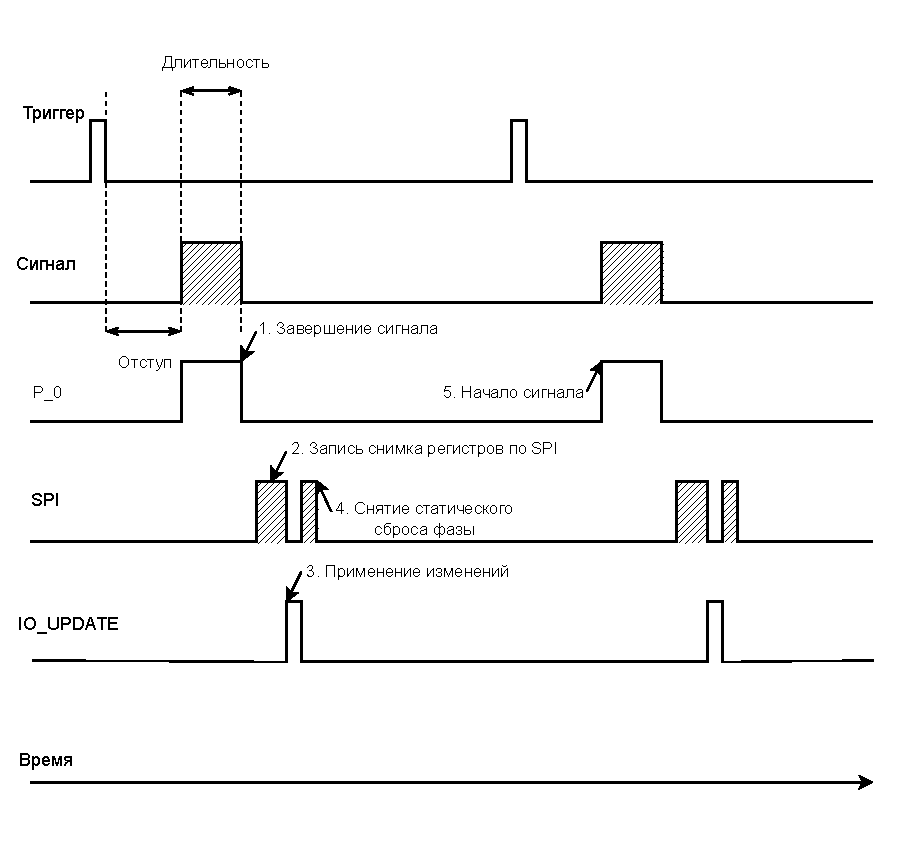
\includegraphics{data/detailed_timing_diagram.drawio.pdf}
\caption{Процедура подачи коротких импульсов.}
\label{fig:detailed_timing_diagram}
\end{figure}
\end{gostfigure}

Показано переключение только одного из входов профилей, поскольку остальные не задействованы и сохраняют низкий уровень. Данная схема верна для сигналов на фиксированной частоте, для ЛЧМ сигналов и для сигналов с модуляцией при помощи оперативной памяти AD9910, но не для сигналов с модуляцией при помощи профилей, где уровни на входах P\_x изменяются в процессе подачи сигнала.

Когда была реализована подача сигналов с произвольными кодовыми последовательностями и FSK/PSK модуляцией при помощи переключения входов профилей, обнаружилась существенная проблема: при одновременном изменении состояния на более чем одном входе P\_x, например при одновременном выставлении высокого уровня на P\_0 и P\_1, синтезатор может выбрать неправильный профиль: несмотря на то, что был выбран профиль 3, с некоторой вероятностью может быть включен как профиль 3, так и профиль 1 либо профиль 2. Точная причина такого поведения не ясна, но скорее всего дело в отсутствии синхронизации переключения профиля относительно тактового сигнала SYNC\_CLK, который внутренне отвечает за опрос всех интерфейсов синтезатора. В даташите явно указано, что уровни на входах профилей должны быть установлены не менее чем за 1.75 нс до фронта SYNC\_CLK, но в текущей реализации это требование не соблюдено и уровни на входах профилей устанавливаются в совершенно произвольные моменты времени относительно SYNC\_CLK. В результате, синтезатор правильно воспринимает только изменение состояния одного входа профилей за один период SYNC\_CLK. Было решено оставить всё так, поскольку это не препятствует реализации подачи сигналов без модуляции или с простой модуляцией, где не требуется переключать более одного входа профилей за раз, например в BPSK.

\subsubsection{Использование AD9910 для ЛЧМ сигналов}

Идеальные ЛЧМ сигналы содержат все частотные составляющие между начальной и конечной частотой, но AD9910 может создавать только конечное множество частот и, следовательно, аппроксимирует ЛЧМ сигналы при помощи дискретных шагов по частоте.

% TODO: Диаграмма отсчёта DRG вверх
Для реализации линейно-частотой модуляции (ЛЧМ) использован блок Digital Ramp Generator (DRG) в AD9910. Блок DRG представляет из себя 32-х битный счётчик, выходное значение которого можно использовать в качестве параметра частоты, амплитуды или фазы сигнала, хотя в случае с амплитудой и фазой задействованы только 16 и 14 младших бит соответственно. Двумя основными параметрами DRG являются значения инкремента и декремента, которые также можно понимать как величину шага по частоте в случае использования DRG в качестве источника значения частоты. Выбор между применением инкремента и декремента, и, соответственно, растущим или убывающим итоговым значением определяется состоянием входа DR\_CTL, где высокий уровень соответствует выбору инкремента, а низкий уровень выбору декремента. Другим ключевым параметром является значение интервала (Ramp Rate) выполнения шагов, которое внутренне является начальным значением для отсчитывающего до нуля таймера. Более высокие значения Ramp Rate соответствуют большему интервалу между шагами, а минимальным полезным значением является 1, когда интервал выполнения шагов составит 4 нс при внутренней частоте AD9910 в 1 ГГц; шагов не будет происходить вообще, если записать ноль в регистр Ramp Rate. Помимо инкремента, декремента и интервала между шагами, можно задать нижнюю и верхнюю границу для выходного значения. Нижняя граница всегда берётся в качестве начального значения счётчика.

Чтобы понять, как ЛЧМ сигналы зависят от параметров DRG, можно рассмотреть частный случай. Если длительность сигнала составляет 900 мкс и значение интервала шагов равно единице, то DRG будет делать шаг каждые 4 нс и сделает 225000 шагов на протяжении всего сигнала. Нужно обратить внимание, что последний шаг будет сделан в момент окончания сигнала, следовательно будет сделано только 224999 видимых инкрементов частоты. Когда значение шага частоты равно единице, один инкремент составляет примерно 0.232 Гц, и полоса сигнала (разница между начальной и конечной частотой) составит примерно 52.386 кГц.

Полосу ЛЧМ сигнала можно выразить следующим псевдокодом:

\lstset{
	language=c,
	basicstyle=\scriptsize\ttfamily,
	numbers=left,
	stepnumber=1,
	showstringspaces=false,
	tabsize=4,
	breaklines=true,
	breakatwhitespace=false,
	xleftmargin=.1\textwidth, xrightmargin=.1\textwidth,
	belowskip=1em, aboveskip=1em
}
\begin{lstlisting}
ceil(duration / 4 ns / b - 1) * (1 GHz / 2^32) * a
\end{lstlisting}

Где значение шага по частоте обозначается как $a$, значение интервала шагов обознается как $b$, а duration --- длительность. Округление вверх добавлено для особых случаев с неполным временем пребывания на конечной частоте. Например, если длительность составляет 16 нс и $b=3$, то синтезатор 12 нс пробудет на начальной частоте, затем 4 нс на изменённой частоте. Если обозначить такие случаи недопустимыми, то округление можно убрать.

Также следует иметь ввиду, что установка верхней границы таким образом, что она будет достигнута до окончания сигнала приведёт к обратному эффекту, когда синтезатор пробудет чрезмерное количество времени на конечной частоте. На рисунке ниже представлено схематичное изображение спектра сигнала в подобной ситуации.

%
% Некоторые частные случаи ЛЧМ сигналов
%
\begin{gostfigure}
\begin{figure}[H]
\centering
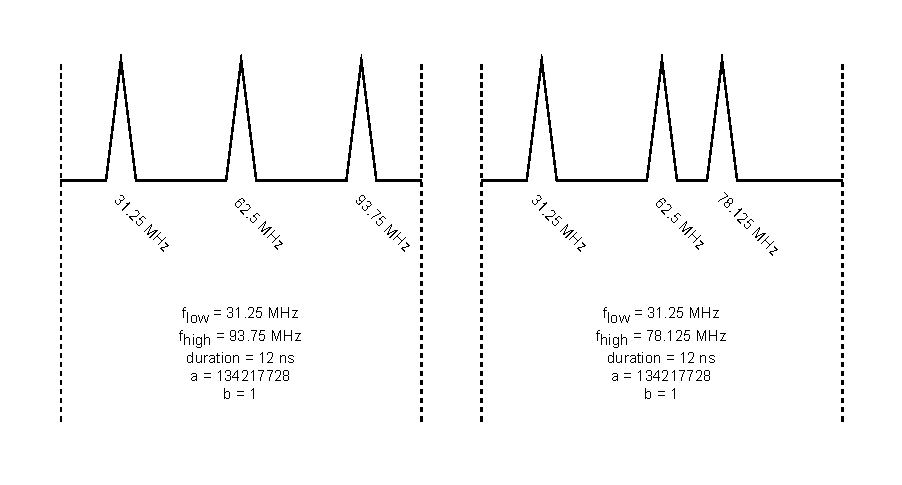
\includegraphics{data/sweep_edge_cases.drawio.pdf}
\caption{Некоторые особые случаи ЛЧМ сигналов.}
\label{fig:sweep_edge_cases}
\end{figure}
\end{gostfigure}

По сравнению с подачей сигналов с фиксированной частотой, подача ЛЧМ сигналов требует дополнительных действий в момент начала подачи сигнала. Во-первых, счётчик DRG должен быть сброшен; для этого доступно два механизма, схожих по принципу действия с механизмами сброса аккумулятора фазы: это сброс по событию, либо статический сброс. Включение статического сброса приведёт к удержанию счётчика в сброшенном состоянии, где значение равно нижней границе. При использовании сброса по событию, изменение состояния входов профилей либо применение IO\_UPDATE приведёт к сбросу счётчика на нижнюю границу. Во-вторых, должен быть сброшен таймер шагов. Он всегда сбрасывается при изменении состояния на входе DR\_CTL, а также может сбрасываться по событию, если выставлен бит Load LRR @ IO Update. В текущей реализации используется сброс счётчика и таймера по событию, что не позволяет использовать модуляцию профилями (в данном случая для изменения амплитуды или фазы) при подаче ЛЧМ сигналов, но модуляция при помощи оперативной памяти остаётся возможной.

Особым случаем является подача ЛЧМ сигналов, где начальная частота выше конечной. Так как стандартными средствами можно произвести сброс только на нижнюю границу, возникает вопрос: как начать ЛЧМ сигнал с верхней границы? Возможным решением является запись значения начальной частоты в регистры нижней и верхней границы одновременно, и выполнение сброса по событию, что должно привести к записи и удержанию значения начальной частоты в счётчике, после чего можно записать значение конечной частоты в регистр нижней границы и применить изменения без сброса. После этого, при смене уровня на вход DR\_CTL на низкий, DRG должен отсчитывать от верхней границы к нижней границе. Данный метод не испытывался, поскольку даташит явно требует, чтобы значение в регистре верхней границы было больше значения в регистре нижней границы, а запись одинаковых значений нарушила бы это условие.

Другим возможным решением является запись значения $2^{32}-1$ в регистр инкремента, что является максимальным возможным значением, выполнение сброса по событию, и ожидание в течение четырёх тактов синтезатора, после чего счётчик выполнит один отсчёт и начнёт удерживать значение верхней границы вместо значения инкремента. Затем, при смене уровня на входе DR\_CTL на низкий в момент начала сигнала, счётчик начнёт отсчитывать с верхней границы к нижней границе. Данный метод тоже не испытывался.

Наконец, ещё одним возможным решением является использование зеркальных частот, которые получаются при значениях $FTW > 2^{31}$ и были рассмотрены в теоретической части этой работы. Так как смысл таких значений $FTW$ меняется, и большие значения соответствуют меньшим частотам, возникает возможность использовать меньшее значение, соответствующее большей начальной частоте, в качестве нижней границы, и наоборот, использовать значение с меньшей частотой в качестве верхней границы. Главной особенностью такого режима работы синтезатора является то, по своему наблюдаемому поведению аккумулятор фазы становится обратным счётчиком, и генерация синусоиды начинается с конца, что выглядит на осциллоскопе как повёрнутая на 180 градусов фаза, что, к счастью, легко компенсируется. В итоге для подачи ЛЧМ сигналов с убывающей частотой был выбран именно этот способ.

Заслуживает упоминания одна дополнительная возможность DRG, которая не проверялась в рамках этой работы --- отсчёт без удержания верхней или нижней границы, когда при достижении верхней границы счётчик мгновенно принимает значение нижней границы, и наоборот, при достижении нижней границы мгновенно принимает значение верхней границы, не прекращая отсчитывать. Возможность использования этого поведения в сочетании с нулевым инкрементом для сброса на верхнюю границу не рассматривалась. В целом, этот режим работы синтезатора, вероятно, предназначен для подачи непрерывных ЛЧМ сигналов, также известных как FMCW, но в рамках данного устройства такие сигналы не представляют интереса.

% TODO: Диаграмма с неудачным свипом

\subsubsection{Использование оперативной памяти AD9910}

Встроенная оперативная память AD9910 способна вместить 1024 32-х битных слова и может использоваться в качестве источника значения частоты, амплитуды, сдвига фазы, либо амплитуды и фазы одновременно, что называется полярным режимом. В режиме источника частоты используются все 32 бита в каждом слове, а в режиме источника фазы или источника амплитуды используются старшие 16 или 14 бит соответственно. В полярном режиме старшие 16 бит отвечают за фазу и последующие 14 бит отвечают за амплитуду, а два оставшихся младших бита не используются.

За выбор адреса в памяти отвечает стейт-машина, у которой есть два основных режима работы: воспроизведение и чтение либо запись. В режиме воспроизведения, в зависимости от настроек, стейт-машина памяти может перемещаться по адресам следующими способами:

\begin{itemize}
	\item Удерживать начальный адрес.
	\item Пройти до конца.
	\item Пройти до конца и обратно.
	\item Циклично ходить до конца.
	\item Циклично ходить до конца и обратно.
\end{itemize}

Указание начального и конечного адреса для воспроизведения осуществляется при помощи регистров профилей, содержимое которых приобретает альтернативный порядок и смысл. Когда используется оперативная память, каждый профиль, помимо начального и конечного адреса, задаёт режим перемещения по адресам и интервал шагов при воспроизведении, о котором можно думать, как о длительности одного элемента. Когда AD9910 работает на тактовой частоте в 1 ГГц, максимальная длительность одного элемента в памяти составляет $65535\times4$ нс $=$ 262.14 мкс. Изменение профиля приводит к сбросу стейт-машины и началу воспроизведения заново.

Чтение и запись оперативной памяти через порт SPI рекомендуется выполнять, пока воспроизведение из оперативной памяти выключено, то есть бит RAM Enable равен нулю. Приведённая в даташите таблица с описаниями битов в регистрах ошибочно утверждает, что бит RAM Enable должен быть выставлен как для воспроизведения, так и для операций чтения и записи, но это не так --- он включает только воспроизведение. Начальный и конечный адрес для операций чтения и записи тоже берутся из регистров профилей, в связи с чем возникает интересная особенность: пока воспроизведение из памяти выключено, используется значение $FTW$ из регистров профилей, а поля начального и конечного адреса памяти пересекаются с полем $FTW$. Для избежания возникновения неожиданных сигналов на выходе синтезатора после установки начального/конечного адреса памяти нужно убедиться, что включен статический сброс фазы или каким-нибудь способом применено нулевое значение амплитуды.

После установки требуемого начального и конечного адреса в регистре любого профиля и выбора соответствующего профиля (или применения изменений, если профиль уже выбран), по интерфейсу SPI производится череда транзакций для считывания или записи одного слова, причём общее количество транзакций должно быть равно разнице между конечным адресом и начальным адресом. Нужно иметь ввиду, что при операциях чтения или записи, счётчик адреса оперативной памяти почему-то работает в обратном режиме, начиная с отсчёт с конечного адреса и отсчитывая до начального.

% TODO: Можно держать восемь разных регионов, но мы этим не пользуемся

Прежде всего оперативная память предназначена для создания сигналов сложной формы, где один из параметров сигнала должен принять более восьми различных состояний за короткий промежуток времени и следовательно не может быть воссоздан при помощи переключения между тремя входами профилей из-за невозможности представить более восьми состояний при помощи трёх входов и также не может быть воссоздан при помощи обновления параметров по SPI из-за ограниченной скорости данного интерфейса.

Значительным преимуществом использования памяти для модуляции по сравнению с переключением профилей является то, что оперативная память позволяет исключить непредсказуемые задержки в моменты переключения элементов кода. При использовании модуляции профилями, переключение элементов кода подвержено двум источникам неопределённости: задержка в переключении GPIO в ответ на события таймера со стороны микроконтроллера, и несколько тактов неопределённости в реакции на переключение профилей со стороны синтезатора, поскольку переключение не синхронизировано с SYNC\_CLK.

Чтобы создать BPSK сигнал с произвольным кодом при помощи оперативной памяти, потребуется сконструировать образ оперативной памяти для этого кода, что было реализовано следующим образом:

\lstset{
	language=c,
	basicstyle=\scriptsize\ttfamily,
	numbers=left,
	stepnumber=1,
	showstringspaces=false,
	tabsize=4,
	breaklines=true,
	breakatwhitespace=false,
	xleftmargin=.1\textwidth, xrightmargin=.1\textwidth,
	belowskip=1em, aboveskip=1em
}
\begin{lstlisting}
vec_t(uint8_t)* vec = scan_uint8_data(str + data_offset);
vec_t(uint8_t)* ram = init_vec(uint8_t);
size_t element_count = vec->size;

for (size_t i = 0; i < element_count; i++) {
	vec_push(ram, 0x7F ? vec->elements[i] : 0x00);
	vec_push(ram, 0xFF ? vec->elements[i] : 0x00);
	vec_push(ram, (ad_default_asf >> 6));
	vec_push(ram, (ad_default_asf << 2) & 0xFF);
}

vec_push(ram, 0x00);
vec_push(ram, 0x00);
vec_push(ram, 0x00);
vec_push(ram, 0x00);

free_vec(vec);
\end{lstlisting}

Здесь на основе разбора кодовой последовательности, состоящей из разделённых пробелами нулей и единиц вида ``0 0 0 1 0'' создаётся образ оперативной памяти в режиме полярной модуляции. Для удобства используется динамический массив. В цикле создаётся 32-х битное слово, верхние 16 бит которого содержат значение 0x7FFF (сдвиг фазы на 180 градусов) или 0x0000 (сдвиг фазы на 0 градусов) в зависимости от значения в кодовой последовательности, а следующие 14 бит всегда содержат одинаковое значение амплитуды. В конец добавляется одно слово с нулевой амплитудой. Таким образом, для кода ``0 0 0 1 0'' получается образ следующего содержания:

\lstset{
	language=c,
	basicstyle=\scriptsize\ttfamily,
	numbers=left,
	stepnumber=1,
	showstringspaces=false,
	tabsize=4,
	breaklines=true,
	breakatwhitespace=false,
	xleftmargin=.1\textwidth, xrightmargin=.1\textwidth,
	belowskip=1em, aboveskip=1em
}
\begin{lstlisting}[firstnumber=0]
0x00 0x00 0xFF 0xFC
0x00 0x00 0xFF 0xFC
0x00 0x00 0xFF 0xFC
0x7F 0xFF 0xFF 0xFC
0x00 0x00 0xFF 0xFC
0x00 0x00 0x00 0x00
\end{lstlisting}

Данный образ затем записывается в оперативную память в момент подготовки к подаче очередного сигнала, после чего настраиваются два профиля: один в режиме прохода от начального адреса 0 до конечного адреса 5, а другой в режиме удержания начального адреса 5, являясь парковочным профилем, активным до начала сигнала и после его завершения. В рамках этого устройства принято использовать нулевой профиль в качестве парковочного и первый профиль в качестве профиля для тела сигнала.

При включении первого профиля и воспроизведении первых пяти элементов из этого образа будет получен BPSK сигнал с заданным кодом, а шестой элемент прервёт сигнал, задав нулевую амплитуду. Через некоторое время микроконтроллер включает парковочный профиль, окончательно завершая цикл подачи сигнала. Так как синтезатор не полагается на внешние события от микроконтроллера для переключения элементов кода и завершения сигнала и автономно отсчитывает время, неопределённости по времени отсутствуют и, форма сигнала приобретает детерминированный вид.

% TODO: Диаграмма

Имея возможность автономно изменять параметры сигнала в зависимости от времени, не полагаясь на медленный внешний микроконтроллер, блок оперативной памяти полезен не только для модуляции, но и для создания точных по длительности сигналов в целом, что было применено для улучшения сигналов с фиксированной частотой и ЛЧМ сигналов относительно их изначальной реализации.

Ранее, для завершения вышеупомянутых сигналов использовалось переключение профилей со стороны микроконтроллера, что вносило примерно 25 нс разброса в общую длительность.

Данный разброс удалось исключить путём использования оперативной памяти для точного по времени обрыва сигнала посредством установки нулевой амплитуды.

Для этого потребовалось реализовать представление произвольных отрезков времени при помощи оперативной памяти. Главная сложность с этим заключается в том, что продолжительность одного элемента в памяти не может превышать 262.14 мкс, и более продолжительные промежутки времени должны быть представлены в виде двух или более элементов.

Чтобы оценить количество необходимых элементов, можно разделить требуемую длительность на 262.14 мкс и округлить вверх, что даст 4 элемента для промежутка длительностью 900 мкс, в случае чего длительность одного элемента должна составлять $\frac{900}{4}=225$ мкс. К сожалению, данная оценка не позволит представить длительность в 901 мкс, где требуемая длительность одного элемента составит $\frac{901}{4}=225.25$ мкс, что не может быть представлено синтезатором, так как не делится на 4 нс. В то же время, длительность в 901 мкс можно представить при помощи пяти элементов, где требуемая длительность одного элемента составит $\frac{901}{5}=180.2$ мкс, что может быть представлено синтезатором.

Был реализован алгоритм поиска перебором, который проверят возможность представления длительности одного элемента, для всех возможных количеств элементов начиная с оценённого минимального значения вплоть до 1023 --- максимального возможного количества элементов в оперативной памяти, с учётом того, что последний будет зарезервирован под завершение сигнала. Ниже представлен программный код, реализующий этот алгоритм:

\lstset{
	language=python,
	basicstyle=\scriptsize\ttfamily,
	numbers=left,
	stepnumber=1,
	showstringspaces=false,
	tabsize=4,
	breaklines=true,
	breakatwhitespace=false,
	xleftmargin=.1\textwidth, xrightmargin=.1\textwidth,
	belowskip=1em, aboveskip=1em
}
\begin{lstlisting}
from math import ceil

def find_element_count(duration_ns):
	start = ceil(duration_ns / 262140)

	for count in range(start, 1024):
		if duration_ns / count % 4 == 0:
			return count

	raise Exception("Unable to represent")
\end{lstlisting}

Данный алгоритм находит, что промежуток длительностью 901 мкс можно представить в виде пяти элементов.

Была встречена интересная проблема, возникающая при использовании блока DRG в сочетании с оперативной памятью при подаче ЛЧМ сигналов с улучшенным отсчётом длительности: начальная фаза в этом режиме была сдвинута в зависимости от начальной частоты. После рассмотрения этого явления на разных частотах стало понятно, что аккумулятор фазы начинает отсчитывать раньше положенного, как будто ненулевое значение $FTW$ начинает поступать аккумулятору фазы существенно раньше, чем ненулевое значение $ASF$ начинает поступать блоку масштабирования амплитуды, что приводит к потере начальной части синусоиды.

При внимательном рассмотрении таблиц задержек внутренних конвейеров в даташите обнаружилось, что значения от DRG действительно поступают на ядро DDS с меньшей задержкой по сравнению с оперативной памятью, даже когда включен режим Matched Latency. Задержка составляет 106 тактов для амплитуды, и 91 такт для частоты, что даёт 15 тактов разницы.

Был реализован механизм компенсации, который на основе начальной частоты прогнозирует фазу по прошествии 15 тактов и находит сдвиг фазы, который необходимо применить к сигналу, чтобы через 15 тактов получилась нулевая фаза. Это не помогло полностью решить проблему --- некоторый сдвиг начальной фазы сохранялся. Экспериментальным путём было установлено, что вычет прогнозируемой спустя 20 тактов фазы позволяет полностью избавиться от смещения начальной фазы на всех частотах. Из этого следует, что в даташите указаны не совсем точные значения задержек.

Из дополнительных особенностей блока оперативной памяти можно выделить режим zero-crossing, который может быть включен или выключен в отдельных профилях и доступен только в режиме удержания начального адреса. Исходя из даташита, этот режим можно применять при создании BPSK сигналов при помощи модуляции профилями, и его функция заключается в задержании применения новых значений сдвига фазы до того момента, когда аккумулятор фазы примет нулевое значение, что позволяет избежать возникновения разрывов в сигнале в момент переключения на противоположную фазу, т.е. переключение фазы происходит с некоторой задержкой от изменения профиля, в ближайший момент, когда синусоида будет находится в нуле. Преимуществом такого сигнала является спектр с меньшим количеством побочных частотных составляющих, но изменение точного момента переключения фазы является недостатком.

Данный режим оказался малополезен из-за серьёзных ограничений относительно частот, на которых задержка остаётся разумной. Когда zero-crossing включен, применение новой фазы может быть задержано на очень большое количество периодов, а не на остаток текущего периода. Это связано с тем, что применение новой фазы задерживается именно до возникновения нуля в аккумуляторе фазы, что происходит сравнительно редко по сравнению с событием обычного переполнения, где остаётся некоторое ненулевое значение. Частота возникновения нулей в аккумуляторе фазы также известна как Grand Repetition Rate и определена как $\frac{F_S}{2^n}$, где $F_S$ это тактовая частота синтезатора, а $n$ --- номер самого младшего ненулевого бита в текущем значении $FTW$. Если требуется, чтобы изменение фазы задерживалось не более чем на 1 мкс, то максимальным допустимым значением $n$ будет 9, но этому условию удовлетворяют всего лишь пять значений $FTW$ из интересующего нас диапазона 154-162 МГЦ.

Нужно отметить, что создавать сигналы с переключением фазы в нуле можно и без этой функции. Если длительность одного элемента в коде соответствует или кратна периоду частоты, то это свойство возникнет само по себе. К сожалению, подобрать такую длительность элементов кода, которая бы кратна периоду 6.49--6.17 нс (целевой диапазон частот устройства), затруднительно. Было решено, что разрывы синусоиды в момент переключения элементов кода при фазовой модуляции являются ожидаемым поведением.

\section*{ЗАКЛЮЧЕНИЕ}
bbb

% Список литературы.
\begin{thebibliography}{11}
\bibitem{DDSTutorial} A Technical Tutorial
on Digital Signal Synthesis https://www.ieee.li/pdf/essay/dds.pdf
\bibitem{STM32F746Datasheet} STMicroelectronics, STM32F746xx Datasheet
\bibitem{NucleoDatasheet} STMicroelectronics, STM32 Nucleo-144 boards (MB1137)
\bibitem{AD9910Datasheet} Analog Devices, AD9910 Datasheet
\bibitem{Kushnarev} Кушнарев Д.С., Лебедев В.П., Хахинов В.В., Евстифеев С.Е., Заруднев В.Е. Модернизация Иркутского радара некогерентного рассеяния. Солнечно-земная физика. 2017. Т. 3, № 3. С. 88-94.
\end{thebibliography}

\appendix

\begin{gostappendix}{Программный код}
\lstset{language=[11]c++,basicstyle=\ttfamily, showstringspaces=false}

\begin{lstlisting}
vvv
\end{lstlisting}
\end{gostappendix}


\begin{gostappendix}{Таблица}
aaa
\end{gostappendix}


\end{document}
